\documentclass[a4paper, 12pt]{article}

\newcommand{\templates}{../../template}
\usepackage[a4paper, margin=2.5cm]{geometry}

\usepackage{enumitem}
\setlist[itemize]{noitemsep}
\setlist[enumerate]{noitemsep}

\let\oldpar\paragraph
\renewcommand{\paragraph}[1]{\oldpar{#1\\}\noindent}
\usepackage{graphicx}
\usepackage{hyperref}
\usepackage{makecell}

\newcommand{\settitolo}[1]{\newcommand{\titolo}{#1\\}}
\newcommand{\setprogetto}[1]{\newcommand{\progetto}{#1\\}}
\newcommand{\setcommittenti}[1]{\newcommand{\committenti}{#1\\}}
\newcommand{\setredattori}[1]{\newcommand{\redattori}{#1\\}}
\newcommand{\setrevisori}[1]{\newcommand{\revisori}{#1\\}}
\newcommand{\setresponsabili}[1]{\newcommand{\responsabili}{#1\\}}
\newcommand{\setversione}[1]{
	\ifdefined\versione\renewcommand{\versione}{#1\\}
	\else\newcommand{\versione}{#1\\}\fi
}
\newcommand{\setdestuso}[1]{\newcommand{\uso}{#1\\}}
\newcommand{\setdescrizione}[1]{\newcommand{\descrizione}{#1\\}}

\newcommand{\makefrontpage}{
	\begin{titlepage}
		\begin{center}

		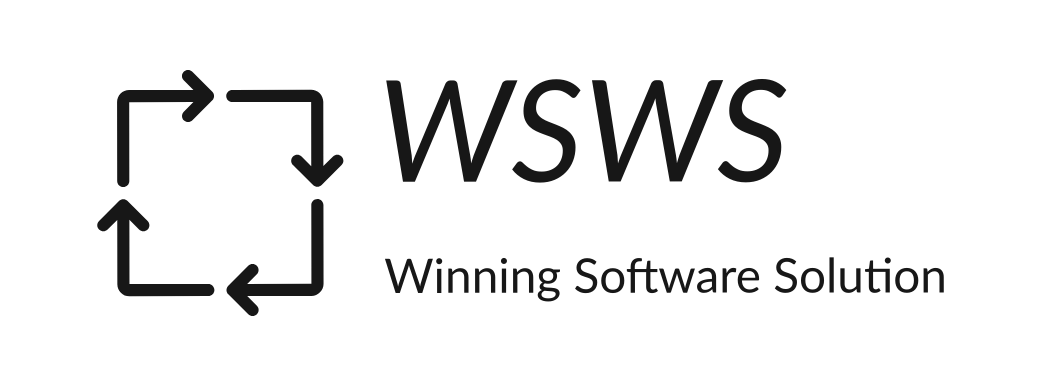
\includegraphics[width=0.4\textwidth]{../../template/WSWS-logos_transparent_crop}\\

		{\Large Winning Software Solution}\\[6pt]
		\href{mailto://winningsoftwaresolution@gmail.com}{winningsoftwaresolution@gmail.com}\\
		
		\ifdefined\progetto
		\vspace{1cm}
		{\Large\progetto}
		{\large\committenti}
		\else\fi
		
		\vspace{1.5cm}
		{\LARGE\titolo}
		
		\vfill
		
		\begin{tabular}{r | l}
		\multicolumn{2}{c}{\textit{Informazioni}}\\
		\hline
		
		\ifdefined\redattori
			\textit{Redattori} &
			\makecell[l]{\redattori}\\
		\else\fi
		\ifdefined\revisori
			\textit{Revisori} &
			\makecell[l]{\revisori}\\
		\else\fi
		\ifdefined\responsabili
			\textit{Respondabili} &
			\makecell[l]{\responsabili}\\
		\else\fi
		
		\ifdefined\versione
			\textit{Versione} & \versione
		\else\fi
		
		\textit{Uso} & \uso
		
		\end{tabular}
		
		\vspace{2cm}
		
		\ifdefined\descrizione
		Descrizione
		\vspace{6pt}
		\hrule
		\descrizione
		\else\fi
		\end{center}
	\end{titlepage}
}
\usepackage{hyperref}
\usepackage{array}
\usepackage{tabularx}

\def\vers#1-#2-#3-#4-#5\\{#1&#2&#3&#4&#5\\\hline}

\newcommand{\addversione}[5]{
	\ifdefined\versioni
		\let\old\versioni
		\renewcommand{\versioni}{#1&#2&#3&#4&#5\\\hline\old}
	\else
		\newcommand{\versioni}{#1&#2&#3&#4&#5\\\hline}
	\fi
}

\newcommand{\setversioni}[1]{\newcommand{\versioni}{#1}}

\newcommand{\makeversioni}{
	\begin{center}
		\begin{tabularx}{\textwidth}{|c|c|c|c|X|}
		\hline
		\textbf{Versione} & \textbf{Data} & \textbf{Persona} & \textbf{Attivtà} & \textbf{Descrizione} \\
		\hline
		\versioni
		\end{tabularx}
	\end{center}
	\clearpage
}

%package
\usepackage[table,xcdraw]{xcolor}

\settitolo{Analisi delle tecnologie}
\setredattori{Federico Marchi \\ Matteo Galvagni}
\setrevisori{Giovanni Cocco}
\setdestuso{Esterno}
\setdescrizione{
Analisi delle tecnologie.
}

\addversione{0.0.0}{data}{chi}{Redazione}{descrizione}

\begin{document}

\makefrontpage

\makeversioni

\section*{Introduzione}
L'infrastruttura designata per questo progetto verte principalmente sulla comunicazione diretta tra attori (clienti/venditori) e blockchain: per rendere utilizzabile il servizio di pagamento non sarà necessario sviluppare solo un contratto digitale che si occupi dello smistamento dei fondi, ma anche una landing page per facilitare il pagamento al cliente ed un servizio di visualizzazione transazioni per entrambi venditori e clienti.
Inoltre, sarà necessario sviluppare uno script per automatizzare la messa in vendita dei prodotti comunicando direttamente in blockchain.
Necessiteremo di un server per fornire la landing page e le pagine di consultazione transazioni, oltre che di un database per memorizzare ID delle transazioni ed altri eventuali dati d'interesse.
Sarà anche necessario fornire un'applicazione mobile (o applicazione web) per il cliente finale e per il corriere al fine di, rispettivamente, sbloccare i fondi e controllare che i fondi siano stati sbloccati.
Per richiamare funzioni nel contratto (quindi eseguire transazioni in blockchain) sarà necessario utilizzare una o più librerie che ci consentano di farlo sia lato server che lato client.

\section*{Blockchain}
La blockchain sulla quale sviluppare il contratto digitale dovrà garantire una velocità di transazione nell'ordine dei secondi e un costo per transazione quanto più basso possibile per garantire una buona usabilità da parte di tutti gli attori coinvolti. In particolar modo, sarà cruciale che lo sblocco dei fondi tramite scannerizzazione del QR sia veloce e poco costoso.
Diverse blockchain sono state prese in esame, ma in conclusione la scelta è ricaduta su Polygon.
Grazie ai suoi costi per transazione molto bassi e la sua finalità di transazione di pochi secondi, la blockchain di Polygon è l'ideale per il tipo di contratto che ci è chiesto di sviluppare.
Inoltre, grazie al suo meccanismo di salvataggio del proprio stato a "checkpoint" su Ethereum, Polygon ne eredita parte della sicurezza.
Polygon è compatibile con la Ethereum Virtual Machine e il suo linguaggio nativo è Solidity. La documentazione esistente per questo linguaggio è esaustiva e facilmente reperibile.
Verrà utilizzata la testnet di Polygon "Mumbai" per lo sviluppo del contratto, in quanto il suo utilizzo è particolarmente comodo e gratuito.

\section*{Backend}
Poiché l'architettura scelta prevede necessariamente l'utilizzo di un server sono state valutate diverse opzioni per quanto riguarda la scelta del linguaggio e dell'eventuale framework per lo sviluppo della parte di backend. Tra questi sono stati presi in considerazione Java e Javascript poiché ci consentono di utilizzare rispettivamente le librerie Web3j e Web3js che permettono di emettere transazioni in blockchain nonchè gestire oggetti (transazione, contratto, ecc) comodamente. La scelta è infine ricaduta sull'utilizzo di TypeScript (NodeJS) poichè ci consente di usufruire della comodità di Javascript (e delle sue librerie che ci interessano) con l'integrazione della tipizzazione. Per l'ascolto di eventi emessi a lato contratto il nodo presso la quale ascoltare sarà fornito dal servizio di API per Polygon "Moralis.io", essendo uno dei pochi nodi che tra l'altro offre un punto di accesso WebSocket e non solamente in HTTPS necessario per la "sottoscrizione" ad eventi in JS.

\section*{Pagamento automatizzato alla messa in vendita}
Per rendere automatizzata la possibilità di pagare un oggetto con ShopChain, durante il normale iter di messa in vendita degli oggetti da parte dei venditori è necessario integrare uno script che dialoghi con la blockchain per creare un'istanza per il pagamento che genererà un ID univoco e conserverà il prezzo atteso per confrontarlo con il denaro inviato di un cliente quando acquisterà tale oggetto.
Tale script verrà sviluppato in Python per comodità di sviluppo e facilità di integrazione. Sarà necessario utilizzare la libreria "Web3py".
Non utilizzando Metamask, il nodo presso la quale emettere le transazioni sarà fornito dal servizio di API per Polygon "Moralis.io".

\section*{Database}
Per la memorizzazione dei dati di nostro interesse circa le transazioni è necessario l'utilizzo di un database. Poiché non sono emerse necessità specifiche per le quali utilizzare un determinato database piuttosto che un altro è stato scelto MariaDB.

\section*{Scansione QR code}
Per quanto riguarda la realizzazione della App/Webapp per lo scansionamento del QR code da parte dei clienti degli Ecommerce, considerando che Metamask su dispositivi mobili non è disponibile sottoforma di estensione per browser ma come intera applicazione con un browser interno dedicato, è stato scelto di sviluppare una Webapp in modo tale che sia comodamente raggiungibile da tale browser interno.

\end{document}
